\documentclass{article}
\usepackage[utf8]{inputenc}
\usepackage{graphicx}
\graphicspath{ {/Users/christin/Desktop/} }

\title{PS6}
\author{Christin Bivens}
\date{March 2018}

\begin{document}

\maketitle


I used data that I am working with for my final project in the class. This data set is about price and characteristics of ready-to-eat cereal and came from a professor at another university. It was relatively clean when I got it, but in order to do manipulation, I needed to clean it a little more.

\begin{itemize}
    \item First, the data set was a .dta file (STATA file). I do not own, nor want to buy STATA. I used the haven package in R to convert the file to .csv. 
    \item Second, I used the tibble package to filter out the parts of the data that I want: The 4 main parent companies who dominate the market: General Mills, Pepsi Co., Kellogg, and those under a Private Label. I know I only need 3 for this assignment, but my research is working with 4, and therefore it seemed like a good opportunity to work on the research
    In order to find the variable names with such a big set I used the sort and unique functions on the Parent Level column, this is not in my shell script as it's not necessary for making the graphs.
    \item Third, I made data frames of the parent company prices and quantities sold.
    \item A quick blind spot on this assignment is that the price data uses e to nth degree, as there are 50,000 data points in the entire set, I am adjusting this in my final project, but not for the assignment. The graphs still show interesting correlation.
    \item Finally, I used ggplot2 to make graphs with price on the vertical axis and quantity on the horizontal axis. this quick visualization lets me see what relationships could be happening, when just looking at a massive spreadsheet my eyes would not be able to give me the same quick overview.
    \item You'll notice that these correlations look fishy, a lot of points on one side. With speculation and research, this is probably a result of coupons being frequent in food purchases, and often after manufacturer coupons many shoppers end up getting money back at the register. This could also be due to the way price is formatted in the data. However, I have made about 50 of these graphs and for some brand names that are subsets of the parent companies, and even for smaller market share parent companies, the graphs look how you would expect them to look. This means, I have a lot of work to do for the final project.
        The graphs looking off does not feel like a failure to me for the first visualization of the data. It tells me that there is something I need to look into that could be a key part of my research conclusions.
\end{itemize}


\includegraphics[scale=.5]{General Mills.png}

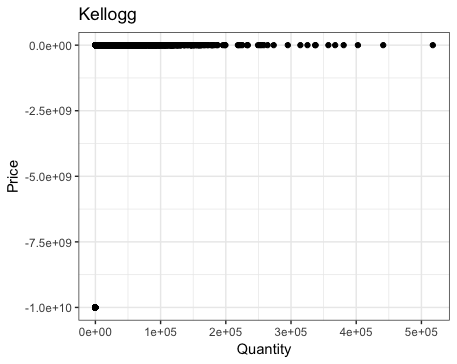
\includegraphics[scale=.5]{Kellogg.png}

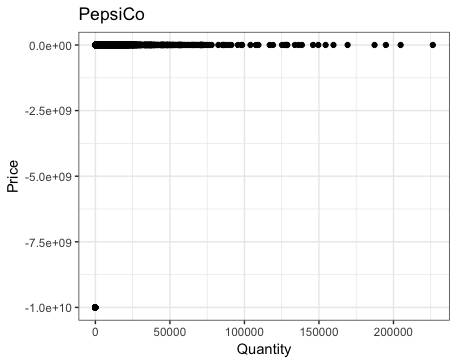
\includegraphics[scale=.5]{PepsiCo.png}

\includegraphics[scale=.5]{Private Label.png}



\end{document}
